%%----------------------------------------------------------------------
%%----------------------------------------------------------------------
\section{Introduction}

\begin{columns}

  \emph{Legacies} is an unofficial, team-oriented skirmish campaign
  for Games Workshop's \emph{Warhammer 40,000}.  Its core is a set of
  eight thematic missions designed for \emph{Recon Squad}, an
  unofficial skirmish variant of \emph{40k} similar to Games
  Workshop's \emph{Kill Team} rules.  Players field only a squad or
  two on a small board with dense terrain, and all their models act
  independently.  It's a very different \emph{40k} experience, focused
  on the heroics of regular grunts, without requiring you to learn new
  core rules.

  Those skirmishes are woven into a campaign here by a set of eight
  Legacies, specific missions the recon squads are striving to
  complete for their alliance.  The campaign climaxes in the
  Cataclysm, in which all the recon squads and some reinforcements
  fight alongside their alliance teammates in a final joint battle.

  \emph{Legacies} may be run either as a single full-day event or over
  several evenings.  Though the missions and legacies are thematic and
  storyful, \emph{Legacies} does not have its own setting, so that it
  can be easily adapted to one of your own making.  Other events are
  also easily connected before or after this campaign to form a larger
  narrative.  Notes are also included here on scoring \emph{Legacies}
  in a narrative tournament or league with individual prizes.

  Recon Squad rules are available here:

  \centerline{\url{rocketshipgames.com/40k/recon-squad/}}

\columnbreak
\noindent\fbox{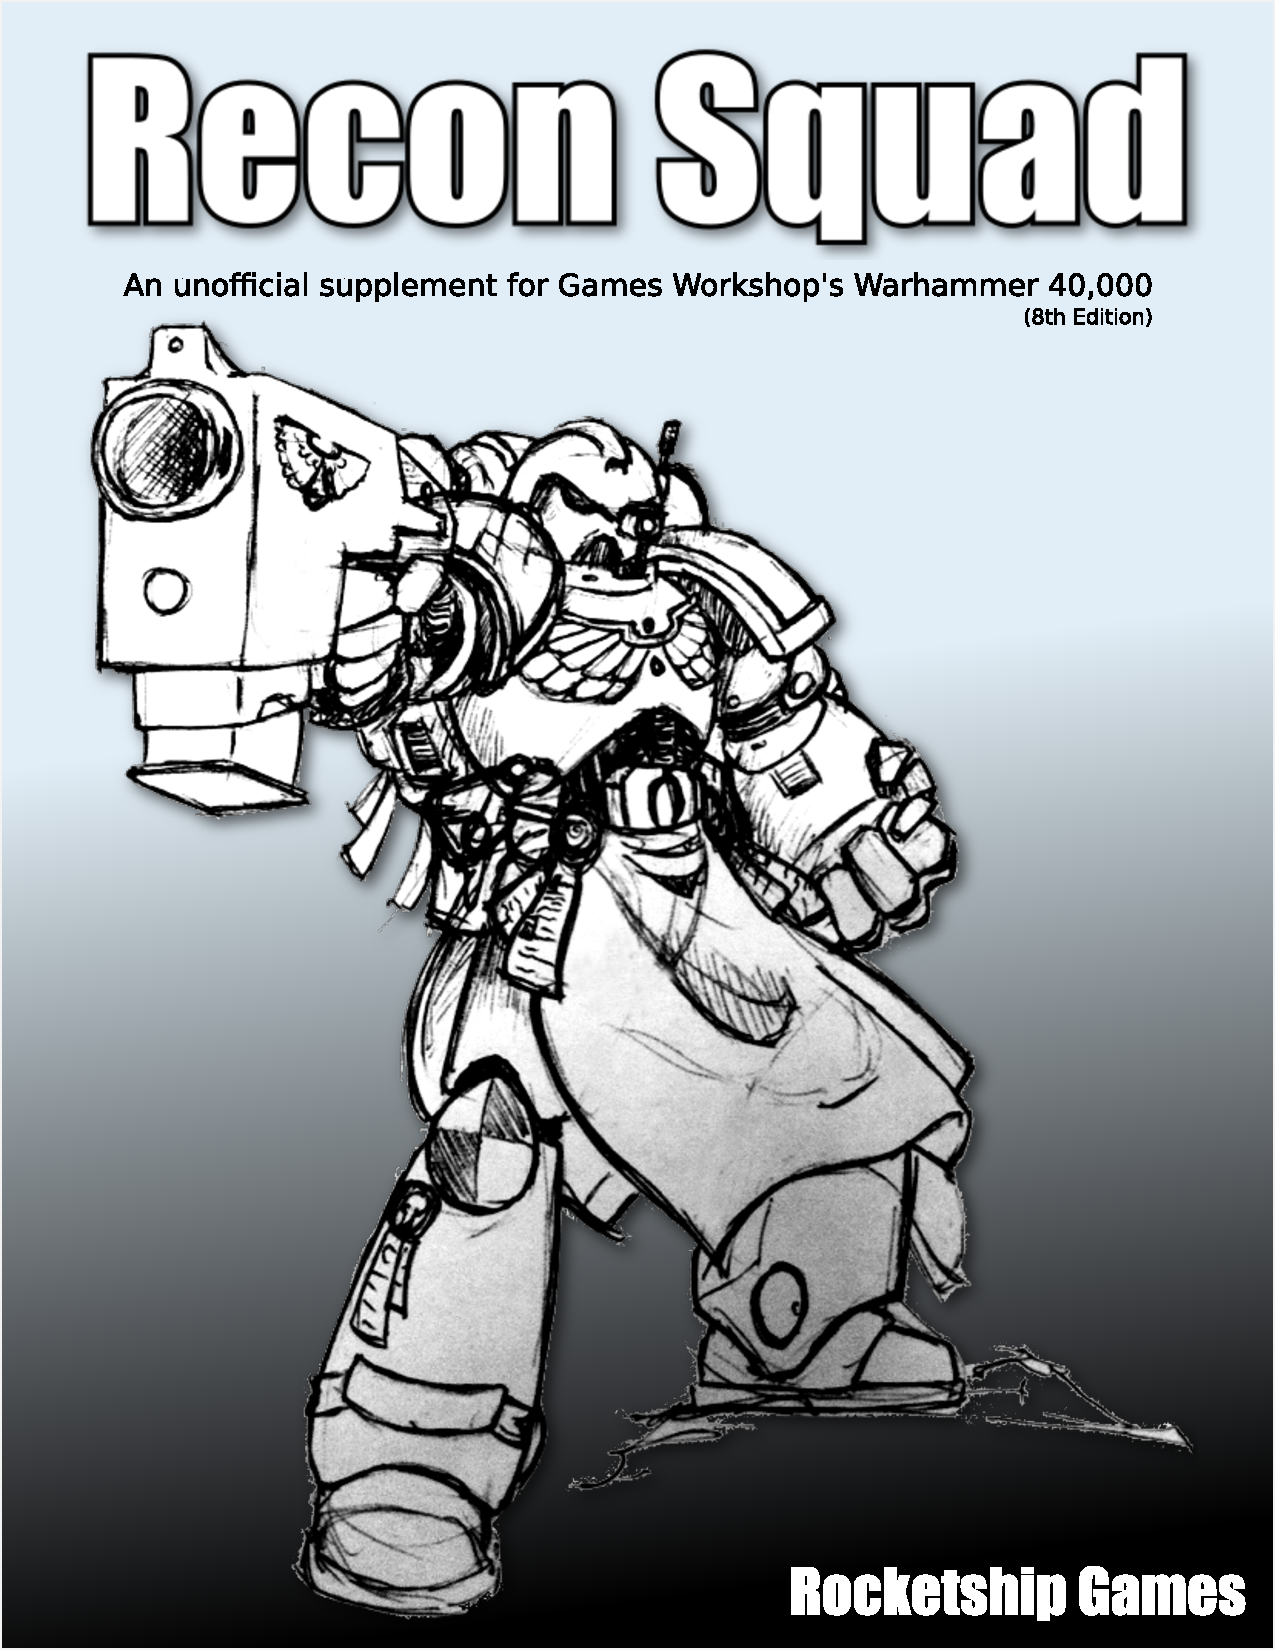
\includegraphics[width=\linewidth]{art/recon-squad_cover.pdf}}
  
\subsection{Overview}

\emph{Legacies} is played as four rounds of Recon Squad skirmishes,
capturing small but pivotal incidents in a larger battle, followed by
a closing Cataclysm team game.

Each player's squad is working toward a legacy within the
greater conflict---

\begin{squishitemize}
\item \textbf{Bodyguards:} Fierce defenders of battlefield
  commanders;

\item \textbf{Excavators:} Daring explorers, technical experts, and
  artifact raiders;

\item \textbf{Headhunters:} Precision instruments of
  targeted violence;
%\end{squishitemize}

  % Following the events of \emph{The Debacle on Caldor IV} it has
  % become clear that the legendary \emph{Scythe of Unbound Light}
  % exists and is immeasurably important.  This discovery has spun the
  % maelstrom of conflict on Caldor IV to even dizzier velocities.
  % Unfortunately, the destruction of the planet is also now inevitable
  % with the Imperium having begun Exterminatus.  With every army
  % shattered and communication all but impossible, it is up to the
  % individual commanders and warriors in the field to rise to the
  % moment.  \emph{The Twilight of Caldor IV} plots the heroics of small
  % bands of warriors furiously moving into position to help their
  % alliance claim the relic before the end.


%\begin{squishitemize}
\item \textbf{Killers:} Shattered fighters disconnected from anything
  but bloodshed;

\item \textbf{Penetrators:} Sharpened blades able to break any
  armor or defense;

\item \textbf{Scouts:} Reckless adventurers reconnoitering the
  battlefield;

\item \textbf{Sentinels:} Implacable defenders and masters of \emph{ad
    hoc} fortifications;

\item \textbf{Warriors:} Hardened veterans that have been through
  everything.
\end{squishitemize}

Their path toward those legacies is defined by the missions they
tackle:

\smallskip\centerline{\begin{tabular}{C{1.5in}C{1.5in}}
\textbf{Ambush} & \textbf{Encirclement}\\
\textbf{Assassination} & \textbf{Excavation}\\
\textbf{Battlefield} & \textbf{Installation}\\
\textbf{Breakthrough} & \textbf{Skirmish}\\
\end{tabular}}

\smallskip%
Successes and failures at those challenges will define both the recon
squad's place in history, and their alliance's ability to win out in
the final Cataclysm.

\end{columns}
